\chapter{Plugin}

Basierend auf den beschriebenen Erkenntnissen wurde ein Plugin für Gephi entwickelt, mit welchem Kanten mit verschiedenen Link Prediction Algorithmen vorhergesagt werden können.
Kanten, welche zum Netzwerk hinzugefügt worden sind, werden entsprechend gekennzeichnet. Die Anzahl vorhergesagter Kanten kann von den Benutzern angegeben werden.
In der Literatur werden hauptsächlich Algorithmen beschrieben, welche auf ungerichtete Graphen anwendbar sind. Algorithmen für gerichtete Graphen weisen eine wesentlich höhere Komplexität auf. Die Arbeit beschränkt sich deshalb auf Link Predictions auf ungerichtete Graphen -
ein entsprechender Hinweis wurde im Gephi Plugin implementiert. Das Plugin enthält zudem eine Evaluationskomponente, mit welcher die Qualität der verschiedenen Algorithmen verglichen werden kann.

Das Plugin wird unter der Apache 2.0 Lizenz veröffentlicht.

\section{Software Architektur}

Das Plugin besteht aus folgenden Hauptkomponenten:

\begin{itemize}
    \item \textbf{Statistik:} Neue Kanten können via Statistiken zu einem ungerichteten Graphen hinzugefügt werden. Für die ausgewählten Algorithmen werden die Link Preditction Werte berechnet und jeweils die Kante mit dem höchsten Wert zum Graphen hinzugefügt. Die Anzahl hinzuzufügender Kanten kann angegeben werden. Die einzelnen Kanten werden dabei iterativ hinzugefügt. Die Berechnung des nächsten vorhergesagten Wertes basiert immer auf dem Graphen des vorherigen Iterationsschrittes.
    \item \textbf{Filter:} Die hinzugefügten Kanten können via Filter angezeigt werden. Dabei können die anzuzeigenden Kanten einerseits auf einen Alorithmus, andererseits auf eine gewünschte Anzahl hinzugefügter Kanten beschränkt werden.
    \item \textbf{Evaluation:} Die Güte der vorhergesagten Kanten kann berechnet werden. Via Statistiken wird die Accurarcy von verschiedenen Algorithmen verglichen und beurteilt.
\end{itemize}

\subsection{Klassenstruktur}
Die Klassenstruktur ist grösstenteils bereits durch das bestehende Grundgerüst von Gephi vorgegeben. Für eine möglichst einfache Erweiterbarkeit, werden entsprechende Design Patterns eingesetzt.

%TODO Refresh UMLs
Abbildung \ref{fig:class_statistic} zeigt das Klassendiagramm der Statistik-Klassen. Es basiert auf dem \acs{compositecommand}\footnote{https://en.wikipedia.org/wiki/Composite\_pattern}, um die Link Prediction Wahrscheinlichkeiten der verschiedenen Algorithmen zu berechnen. Das Composite Pattern beruht darauf, in einer abstrakten Klasse sowohl konkrete Objekte als auch ihre Behälter zu repräsentieren. Damit können sowohl einzelne Objekte als auch ihre Kompositionen einheitlich behandelt werden (\cite{noauthor_kompositum_2019}). Das Makro Command Objekt \texttt{LinkPredictionMacro} wird eingesetzt, um die Kennzahlen von mehreren ausgewählten Algorithmen zu berechnen.
\begin{figure}
    \centering
    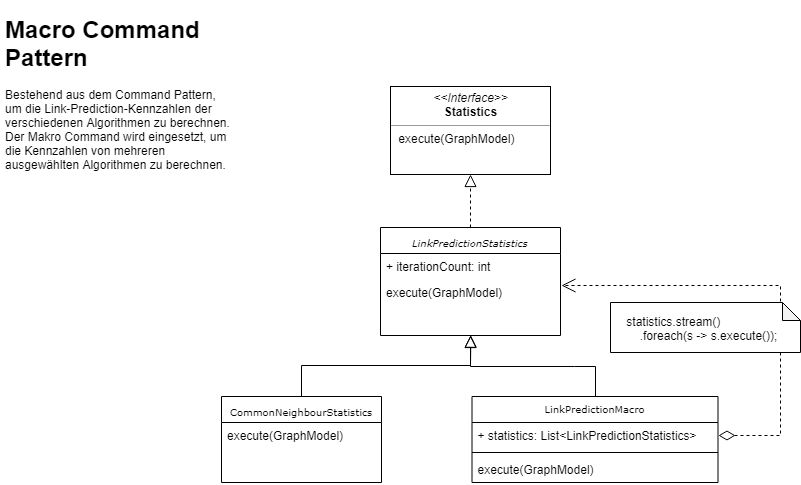
\includegraphics[width=\linewidth]{resources/class_Statistic.png}
    \caption{Klassendiagramm Statistiken}
    % TODO Add cite to SNA Script
    \label{fig:class_statistic}
\end{figure}

Bei der \texttt{execute}-Methode wird auf das \acs{templatepattern}\footnote{https://de.wikipedia.org/wiki/Schablonenmethode} zurückgegriffen. Mit dem Template Pattern kann eine Grundstruktur eines Algorithmus vorgegeben werden, wobei Unterklassen ermöglicht wird, bestimmte Schritte des Algorithmus zu überschreiben ohne dessen grundlegende Struktur zu verändern.
Das Pattern wird hier verwendet, um die unveränderlichen Teile eines Algorithmus einmalig zu implementieren, doppelten Code zu reduzieren, und die Erweiterungen der Unterklassen zu regulieren.
In der \texttt{execute}-Methode wird der grobe Ablauf umschrieben.
Dieser sieht vor, dass bei der initialen Berechnung der Link Prediction Werte sämtliche Knoten zweimal durchlaufen werden müssen.
Beim Ausführen der Link-Prediction kann angegeben werden, wieviele Kanten hinzugefügt werden sollen.
Aus Performancegründen erwies es sich als sinnvoll, für die nachfolgenden Berechnungen nicht mehr sämtliche Werte nochmals zu berechnen.
Stattdessen wird nach dem Hinzufügen einer Kante im nächsten Iterationsschritt nur die davon betroffenen Knoten neu berechnet.
Falls beispielsweise eine Kante $(A, C)$ zum Graphen hinzugefügt wird, müssen anschliessend nur die Werte der Knoten $A$ und $C$ neu berechnet werden.
Die \texttt{execute}-Methode entält deshalb den groben Ablauf, welcher die Unterscheidung zwischen initialem Durchlauf und nachfolgender Neuberechnung vorsieht.
Die Methoden \texttt{calculateAll} und \texttt{recalculateAffected}, die von den konkreten Klassen implementiert werden und die effektiven Link Prediction Werte berechnent, werden als abstrakt definiert.
Das Listing \ref{lstLinkPrediction} zeigt die vereinfachte Struktur der Methode.

%TODO: Make sure naming e.g. calculate is correct
\begin{lstlisting}[caption={Link prediction implementation},label=lstLinkPrediction]
    // LinkPredictionStatistics.java
    @Override public void execute(GraphModel graphModel) {

        if (isInitialExecution()) {
            // Iterate over all nodes for first iteration
            calculateAll(Graph graph)
        } else {
            // Only change affected node for subsequent iterations
            recalculateAffectedNodes(factory);
        }

        // Add highest predicted edge to graph
        addHighestPredictedEdgeToGraph(factory, getAlorithmName());

    }
\end{lstlisting}

Eine ähnliche Struktur wird bei der Evaluationskomponente verwendet.
Die Qualität der verschiedenen Algoirthmen wird mit der bereits eingeführten Accuracy (vgl. Formel \ref{eq:acc}) bestimmt.
Damit das Plugin später einfach um andere Evaluationsmetriken erweitert werden kann, wurde eine neue Basisklasse \texttt{EvaluationMetric} eingeführt.
Diese enthält den zu evaluierenden Algorithmus, die Berechnung der Kennzahl und die erreichte Güte der Vorhersage. Konkrete Evaluationsmetriken, wie \texttt{LinkPredictionAccuracy} erweitern die abstrakte Basisklasse mit einer konkreten Implementierung der \texttt{calculate}-Methode.
Abbildung \ref{fig:class_eval} zeigt das vereinfachte Klassendiagramm der Evaluation-Klassen.
\begin{figure}
    \centering
    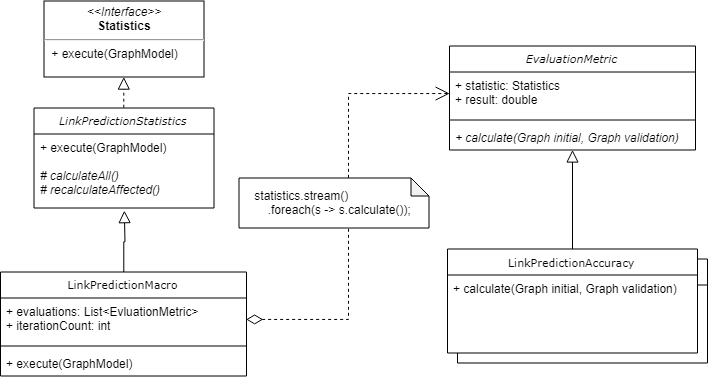
\includegraphics[width=\linewidth]{resources/class_Evaluation.png}
    \caption{Klassendiagramm Evaluationskomponente}
    % TODO Add cite to SNA Script
    \label{fig:class_eval}
\end{figure}

Die Filter-Klassen wurden mithilfe des \acs{abstractfactory}\footnote{http://www.hsufengko.com/blog/abstract-factory-design-pattern-example} umgesetzt. Die Klassenstruktur besteht aus dem Factory Pattern mit verschiedenen Builder Klasse und dem Strategy Pattern, welches eine spezifische Umsetzung der Filter pro Algorithmus erlaubt. Abbildung \ref{fig:class_filter} zeigt das resultierende Klassendiagramm.
\begin{figure}
    \centering
    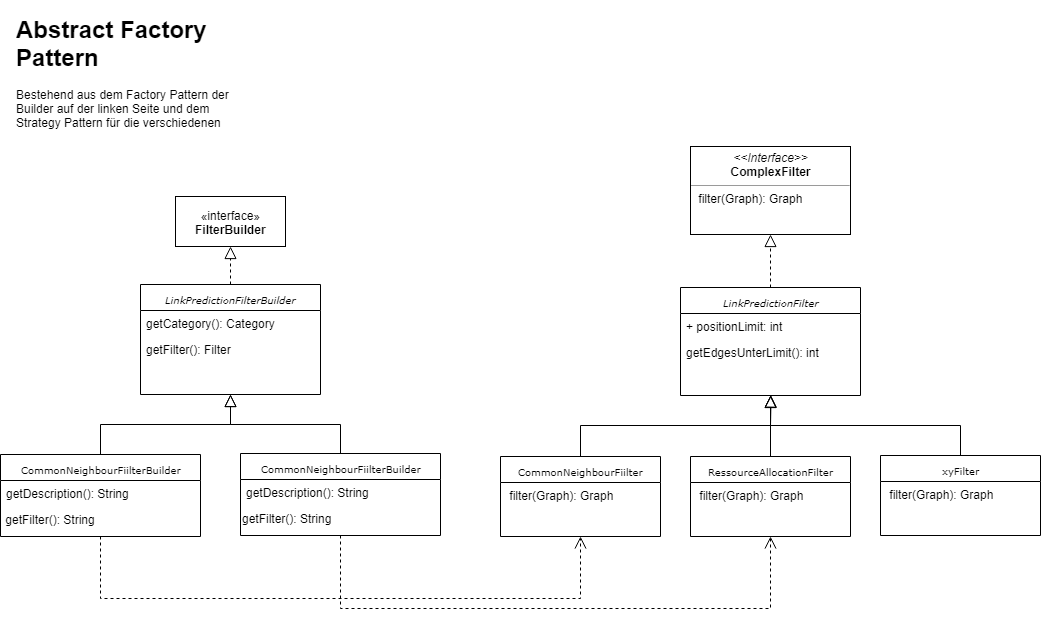
\includegraphics[width=\linewidth]{resources/class_Filter.png}
    \caption{Klassendiagramm Filter}
    % TODO Add cite to SNA Script
    \label{fig:class_filter}
\end{figure}

\subsection{Loggingkonzept}
\label{loggingkonzept}

Im Plugin wird das Logging-Framework log4j\footnote{https://logging.apache.org/log4j/2.x/} eingesetzt.
Das Logging wird eingesetzt um technische Probleme rückverfolgen zu können: Die Logs zeichnen Ereignisse auf, die für die Entwicklung und den Einsatz des Plugin von Nutzen sein können.
Insbesondere geht es darum ein Fehlverhalten der Applikation nachvollziehen und dokumentieren zu können.

\textbf{Logger erzeugen}
Logger sind für das Verfassen von Meldungen verantwortlich. Sie werden direkt aus dem Code aufgerufen und bestimmen mit Hilfe von Appendern wohin und in welchem Format die Meldungen geschrieben werden.
Für jede Klasse wird ein separater Logger erzeugt. Das Codelisting \ref{lstLoggerCreate} zeigt, wie ein solcher Logger in der gewünschten Klasse erzeugt wird.

\begin{lstlisting}[caption={Erzeugen eines Loggers},label=lstLoggerCreate]
    import org.apache.log4j.Logger;

    /**
    * ...
    */
    public class LinkPredictionStatistics \{

    // Console Logger
    private static Logger consoleLogger = LogManager.getLogger(LinkPredictionStatistics.class);
\end{lstlisting}

\textbf{Log-Einträge erzeugen}
%TODO: Add Log4j to Glossar
Log4j bietet verschiedene Log-Levels an, mit welchen Log-Einträge geschrieben werden können.
Tabelle \ref{tab_log_levels} zeigt die verschiedenen Log-Levels anhand der \acs{API}-Docs von log4i:

\begin{table}[]
    \centering
    \resizebox{\textwidth}{!}{%
    \begin{tabular}{@{}ll@{}}
        \toprule
        Level & Beschreibung                                                                                                                                                       \\ \midrule
        TRACE & The TRACE Level designates finer-grained informational events than the DEBUG                                                                                       \\
        DEBUG & \begin{tabular}[c]{@{}l@{}}The DEBUG Level designates fine-grained informational events that are most useful\\  to debug an application.\end{tabular}              \\
        INFO  & \begin{tabular}[c]{@{}l@{}}The INFO level designates informational messages that highlight the progress of the\\ application at coarse-grained level.\end{tabular} \\
        WARN  & The WARN level designates potentially harmful situations.                                                                                                          \\
        ERROR & \begin{tabular}[c]{@{}l@{}}The ERROR level designates error events that might still allow the application to con-\\ tinue running\end{tabular}                     \\
        FATAL & \begin{tabular}[c]{@{}l@{}}The FATAL level designates very severe error events that will presumably lead the \\ application to abort.\end{tabular}                 \\ \bottomrule
    \end{tabular}%
    }
    \caption{Logging-Levels}
    \label{tab_log_levels}
\end{table}

Grundsätzlich kann direkt mit den Funktionen auf dem Logger-Objekt (z.B. \texttt{trace}, \texttt{debug}, etc.) geloggt werden.
Falls in der Log-Meldung Variabeln ausgewertet werden, empfiehlt sich jedoch die Lambda schreibweise mit Lazy-Evaluation.
Listing \ref{lstLoggerUse} zeigt zwei solcher Beispiele.

\begin{lstlisting}[caption={Log-Einträge erzeugen},label=lstLoggerUse]
    public int getNextIteration(Graph graph, String algorithm) {
    consoleLogger.trace("Lookup next iteration");
    int lastIteration;
    // do some lookups here

    consoleLogger.log(Level.DEBUG, () -> "Number of last iteration: " + lastIteration);
    }
\end{lstlisting}

\textbf{Logger Hierarchie}
Alle Logger der verschiedenene Klassen erben vom Root-Logger. Über diesen kann die Konfiguration für alle Logger geändert werden.
Einzelne Logger können die Root-Konfiguration bei Bedarf übersteuern.

\textbf{Appender}
Aktuell wird im Plugin hautpsächlich der \texttt{ConsoleAppender} eingesetzt.
Mit dessen Hilfe kann direkt in die Gephi-Konsole geloggt werden.

\textbf{Konfiguration}

\begin{lstlisting}[caption={log4j.xml},label=lstLoggerCreate]
    <?xml version="1.0" encoding="UTF-8" ?>
    <Configuration>
    <Appenders>
    <Console name="console" target="SYSTEM_OUT">
    <PatternLayout pattern="%d{HH:mm:ss} %-5p %L [%C] - %m%n"/>
    </Console>

    <Loggers>
    <Logger name = "org.gephi.plugins.linkprediction.statistics.PreferentialAttachmentStatistics" additivity="false">
    <AppenderRef ref="console" />
    </Logger>

    <Root level="INFO" additivity="false">
    <AppenderRef ref="file" />
    </Root>
    </Loggers>

    </Configuration>
\end{lstlisting}

\section{Exception-Handling}
\label{exceptionhandling}

Beim Handling von unerwarteten Situation wird zwischen Exceptions und Errors unterschieden.

Exceptions sind unerwartete Zustände, bei deren das Plugin weiterlaufen kann. Allenfalls ist dabei eine Handlung des Benutzers erforderlich.
In solchen Situationen wird dem Benutzer ein Pop-up Fenster mit einem entsprechenden Hinweis angezeigt.
Im Plugin existiert dafür die Basisklasse \texttt{LinkPredictionWarning}, welche durch die konkreten Warning-Klassen erweitert wird.
Im Gegensatz zu Exceptions tritt bei Errors hingegen ein Fehler auf, der ein korrektes Weiterlaufen des Plugins verhindert.
In diesem Fall wird auf das Gephi-interne Exception-Handling zurückgegriffen und der Stacktrace dem Benutzer angezeigt.

\section{GUI Konzept}

Die Link Prediction Funktionalität soll möglichst gut in die bestehende Gephi Benutzeroberfläche integriert werden.
Bei der Analyse der bestehenden \acs{ui}-Elemente stellten sich die folgenden Punkte heraus:
:

\begin{itemize}
    \item Unter dem Menü-Punkt \ovalbox{Statistics} werden diverse Werte des Graphen berechnet und gegebenenfalls im Data Laboratory
          hinzugefügt. Die Darstellung der Ergebniswerte erfolgt über einen Report, sofern sinnvoll.
    \item Unter dem Menü-Punkt \ovalbox{Filter} werden lediglich bereits vorhandene Daten, gefiltert. Hierbei werden Graphen für gewöhnlich verkleinert dargestellt, also mit weniger Kanten oder Knoten.
    \item Die Darstellung der verschiedenen Werte wird über den Menü-Punkt \ovalbox{Appearance} vorgenommen. Hier können Farben,
          und Grösse der Knoten und Kanten eingestellt werden. Beim Filtern werden keine neuen Werte berechnet oder generiert.
    \item Im \ovalbox{Data Laboratory} sind die aktuellen Daten zu finden. Werden neue Daten über Statistics berechnet
          oder die Daten im Laboratory verändert, werden nur die neusten Daten angezeigt. Um alte Daten zu erhalten,
          muss bei jeder Änderung ein neuer Workspace erstellt werden.
\end{itemize}

Das \acs{gui}-Konzept des Link Prediction Plugins basiert auf diesen Grundkonzepten.

\subsection{Vorhersagen neuer Kanten}

Die Berechnung der neuen Kanten muss im Bereich der \ovalbox{Statistics} passieren, da hier neue Werte berechnet und dem
Data Laboratory hinzugefügt werden. Im Folgenden wird dieser Vorgang beschrieben:

\begin{figure}
    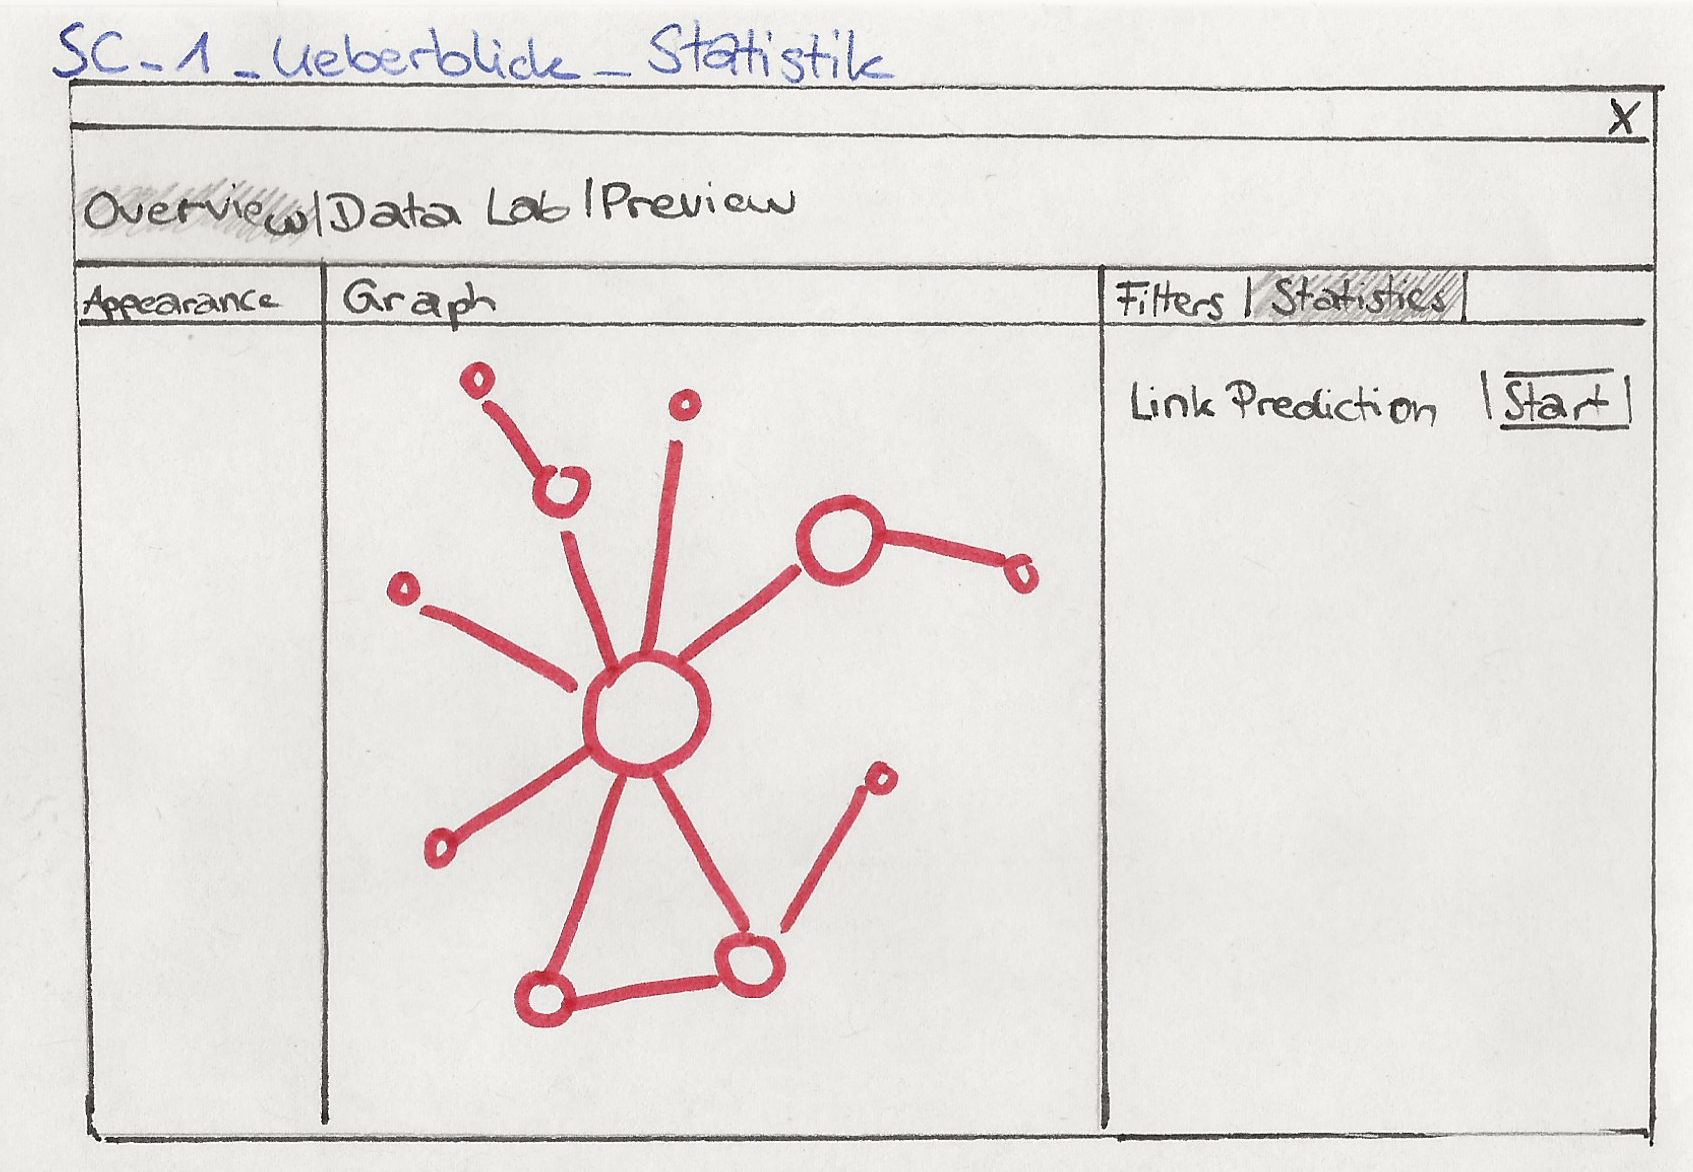
\includegraphics[width=\linewidth]{resources/SC-1.png}
    \caption{Überblick der Ansicht Statistik.}
    \label{fig:screen1}
\end{figure}

Abbildung \ref{fig:screen1} zeigt einen Überblick über die Benutzeroberfläche von Gephi. Grau hinterlegt sind die
angewählten Menü-Punkte. Unter dem Menü \ovalbox{Statistics} wird hier nun ein Element ``Link Prediction'' mit einem
Start-Button eingefügt. Um die Darstellung auf die wesentlichen Elemente zu reduzieren, wurden bestehende Statistiken
nicht eingezeichnet.

\begin{figure}
    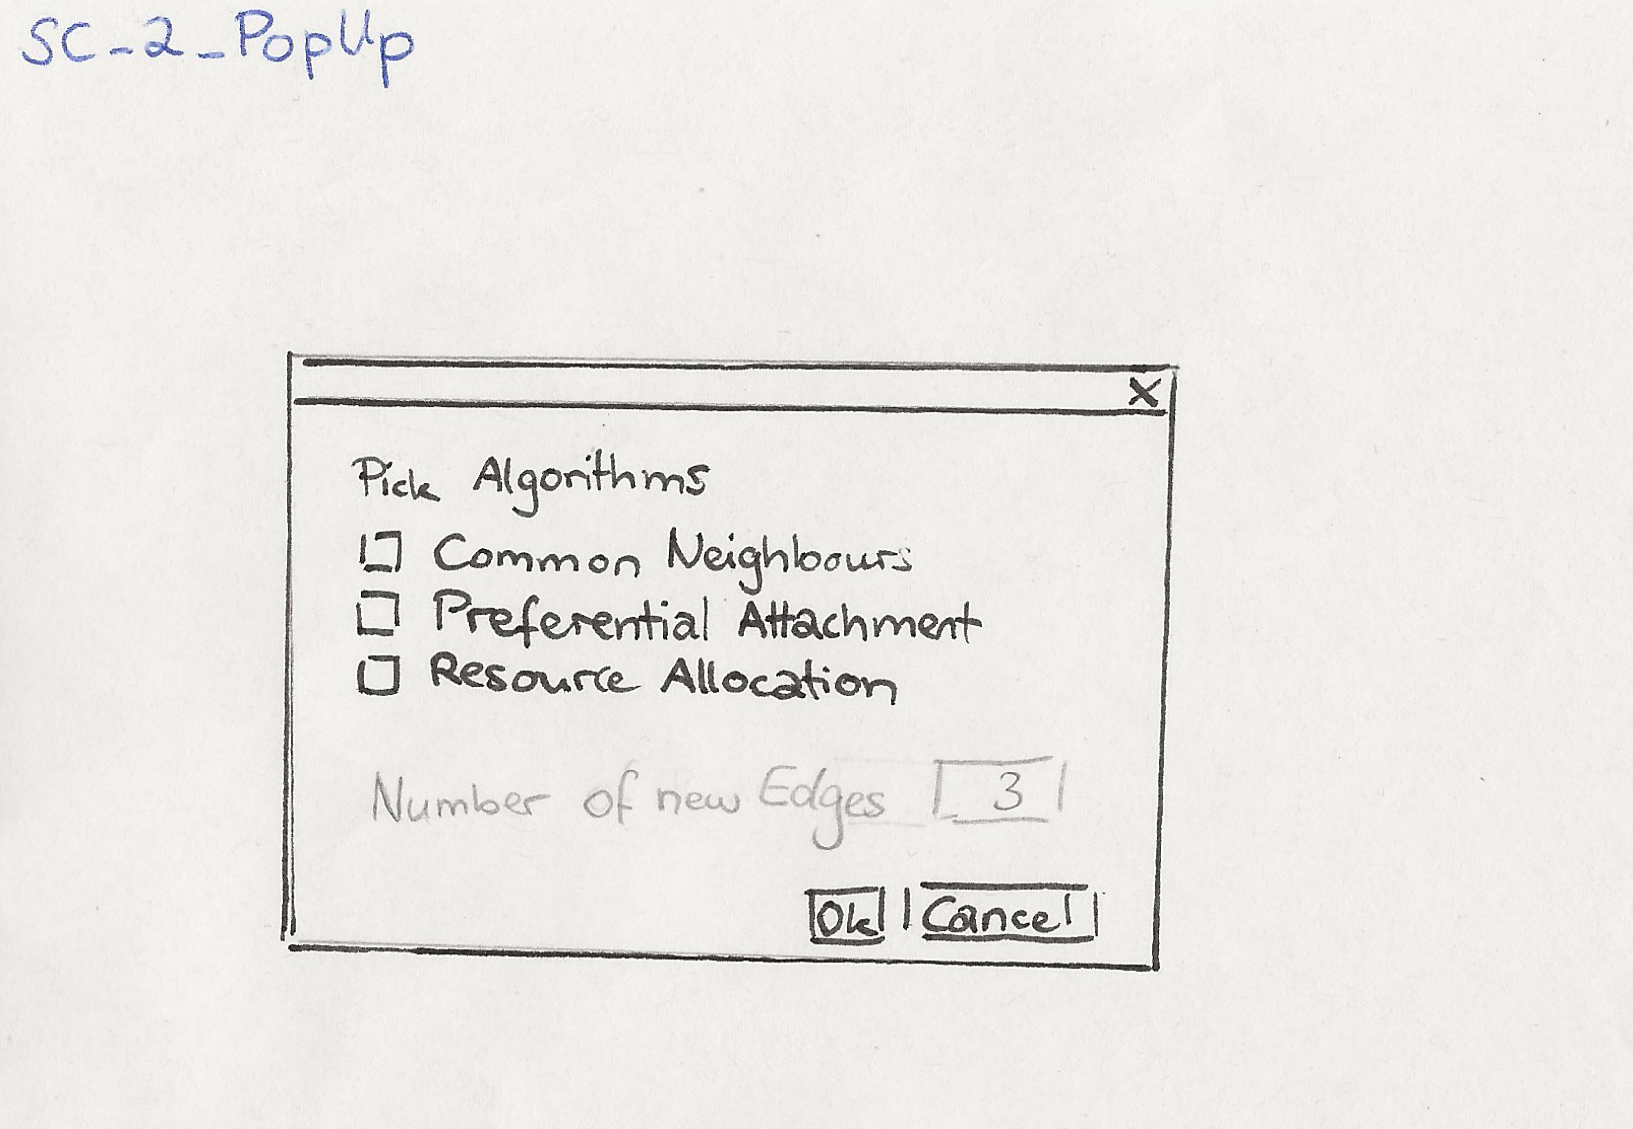
\includegraphics[width=\linewidth]{resources/SC-2.png}
    \caption{Pop-Up für die Auswahl der Berechnung.}
    \label{fig:screen2}
\end{figure}

Falls die \ovalbox{Start}-Schaltfläche angewählt wird, öffnet sich ein Pop-up Fenster, in welchem man verschiedene Algorithmen auswählen
kann. Für alle ausgewählten Algorithmen, werden Link Predictions durchgeführt. Abbildung \ref{fig:screen2} zeigt das Pop-up für die Auswahl der Berechnung. Weitere Informationen zum jeweiligen Algorithmus werden angezeigt, wenn mit der Maus über das entsprechende Element gefahren wird. In einem zusätzlichen Eingabefeld kann man einen Wert
$>= 1$ eingeben. Dieser besagt, wie viele Durchgänge bei der Link Prediction gemacht werden sollen, respektive wie viele
neue Kanten dem Graphen hinzugefügt werden.

Die einzelnen Kanten werden iterativ zum Graphen hinzugefügt. Die Berechnung des nächsten vorhergesagten Wertes basiert immer auf dem Graphen des vorherigen Iterationsschrittes.

\item \textbf{Filter:} Die hinzugefügten Kanten können via Filter angezeigt werden. Dabei können die anzuzeigenden Kanten einerseits auf einen Alorithmus, andererseits auf eine gewünschte Anzahl hinzugefügter Kanten beschränkt werden.

% TODO: Weglassen?
%Die Funktion der zusätzlichen Konfiguration eines Algorithmus ("advanced" Button) wird offen gehalten, wird aber für die
%Implementierung des Common Neighbour und Preferential Attachment Algorithmus derzeit nicht benötigt.

Ein grosses Netzwerk oder auch eine hohe Anzahl an Iterationen kann in einer grossen Laufzeit resultieren.
In diesem Fall soll eine Warnung an den User ausgegeben
werden. Wird diese bestätigt, so wird der Algorithmus trotzdem berechnet. Beim Abbruch kann der User seine gewünschten
Parameter nochmals verändern.

\begin{figure}
    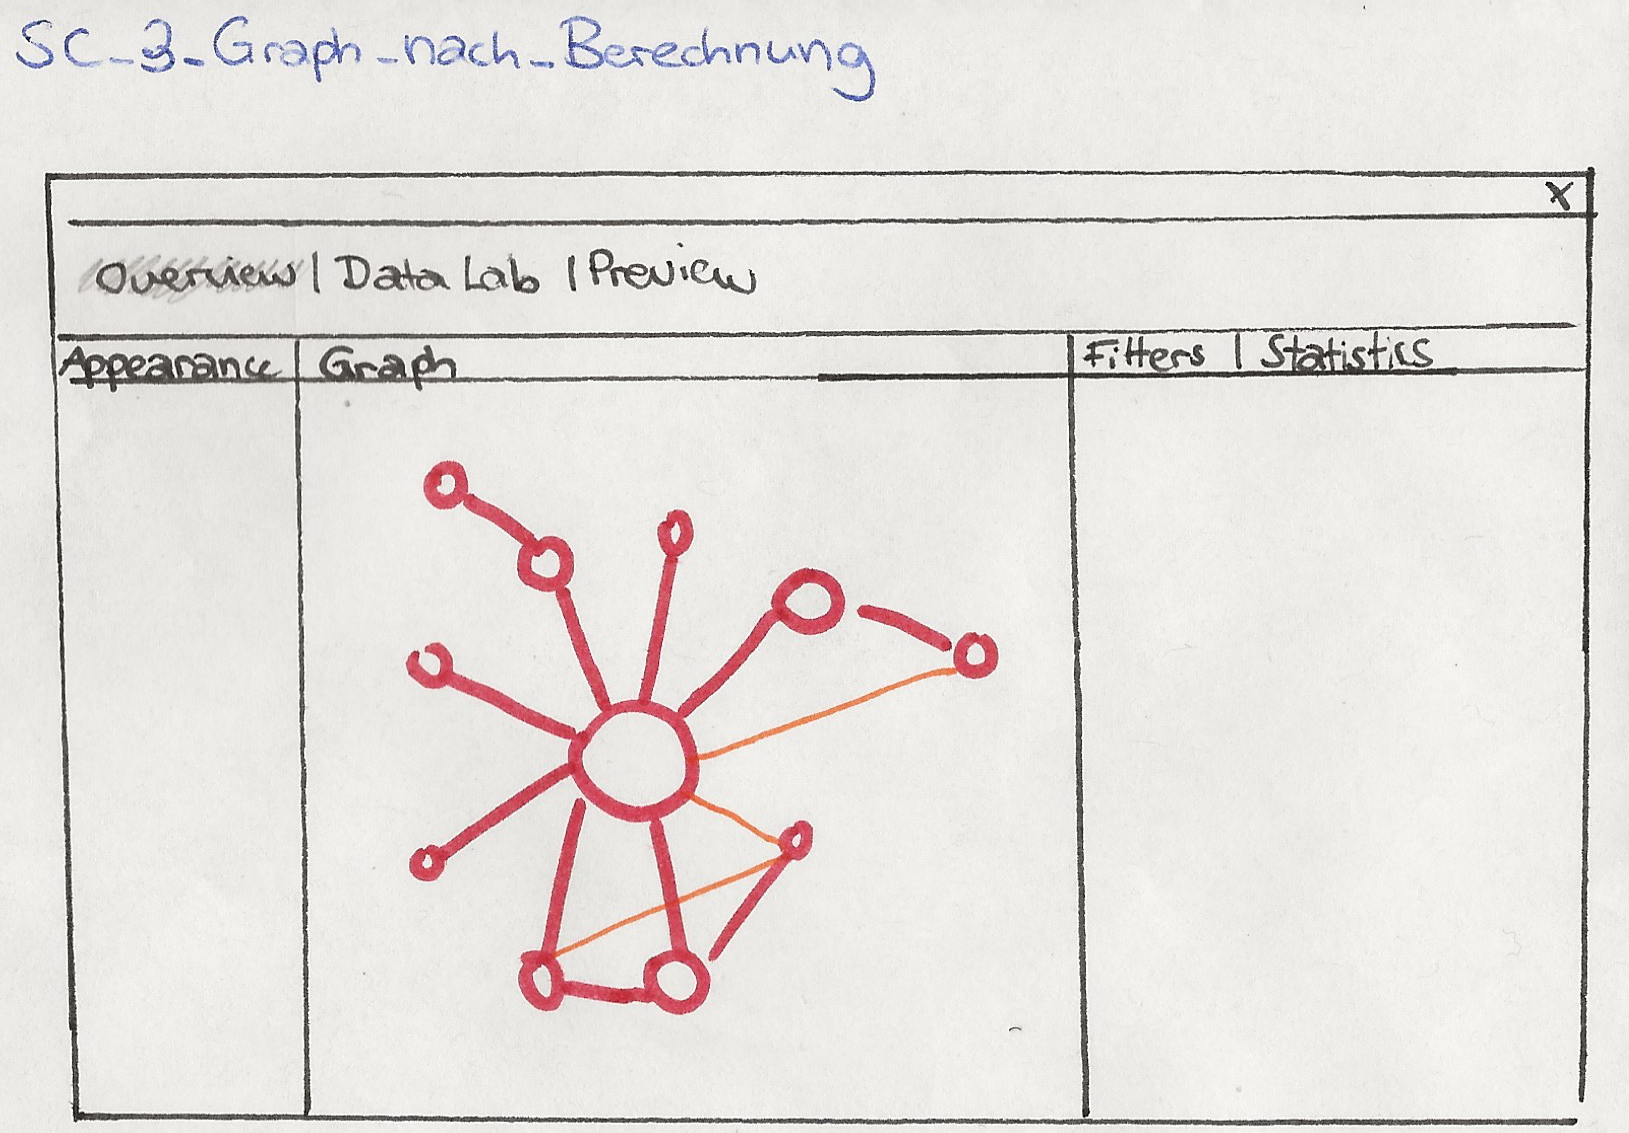
\includegraphics[width=\linewidth]{resources/SC-3.png}
    \caption{Modifizierter Graph mit vorhergesagtem Edge.}
    \label{fig:screen3}
\end{figure}

Abbildung \ref{fig:screen3} zeigt den Graph nach der Berechnung Link Predictions.
Gegenüber dem initialen Graphen wurden neue Kanten hinzugefügt.
Diese können mit Hilfe der Appearance-Einstellungen eingefärbt werden, da im Data Laboratory Felder enthalten sind, die aussagen, ob eine
Kante mit einem Link Prediction Algorithmus hinzugefügt wurde oder ob sie bereits existiert hat.

\begin{figure}
    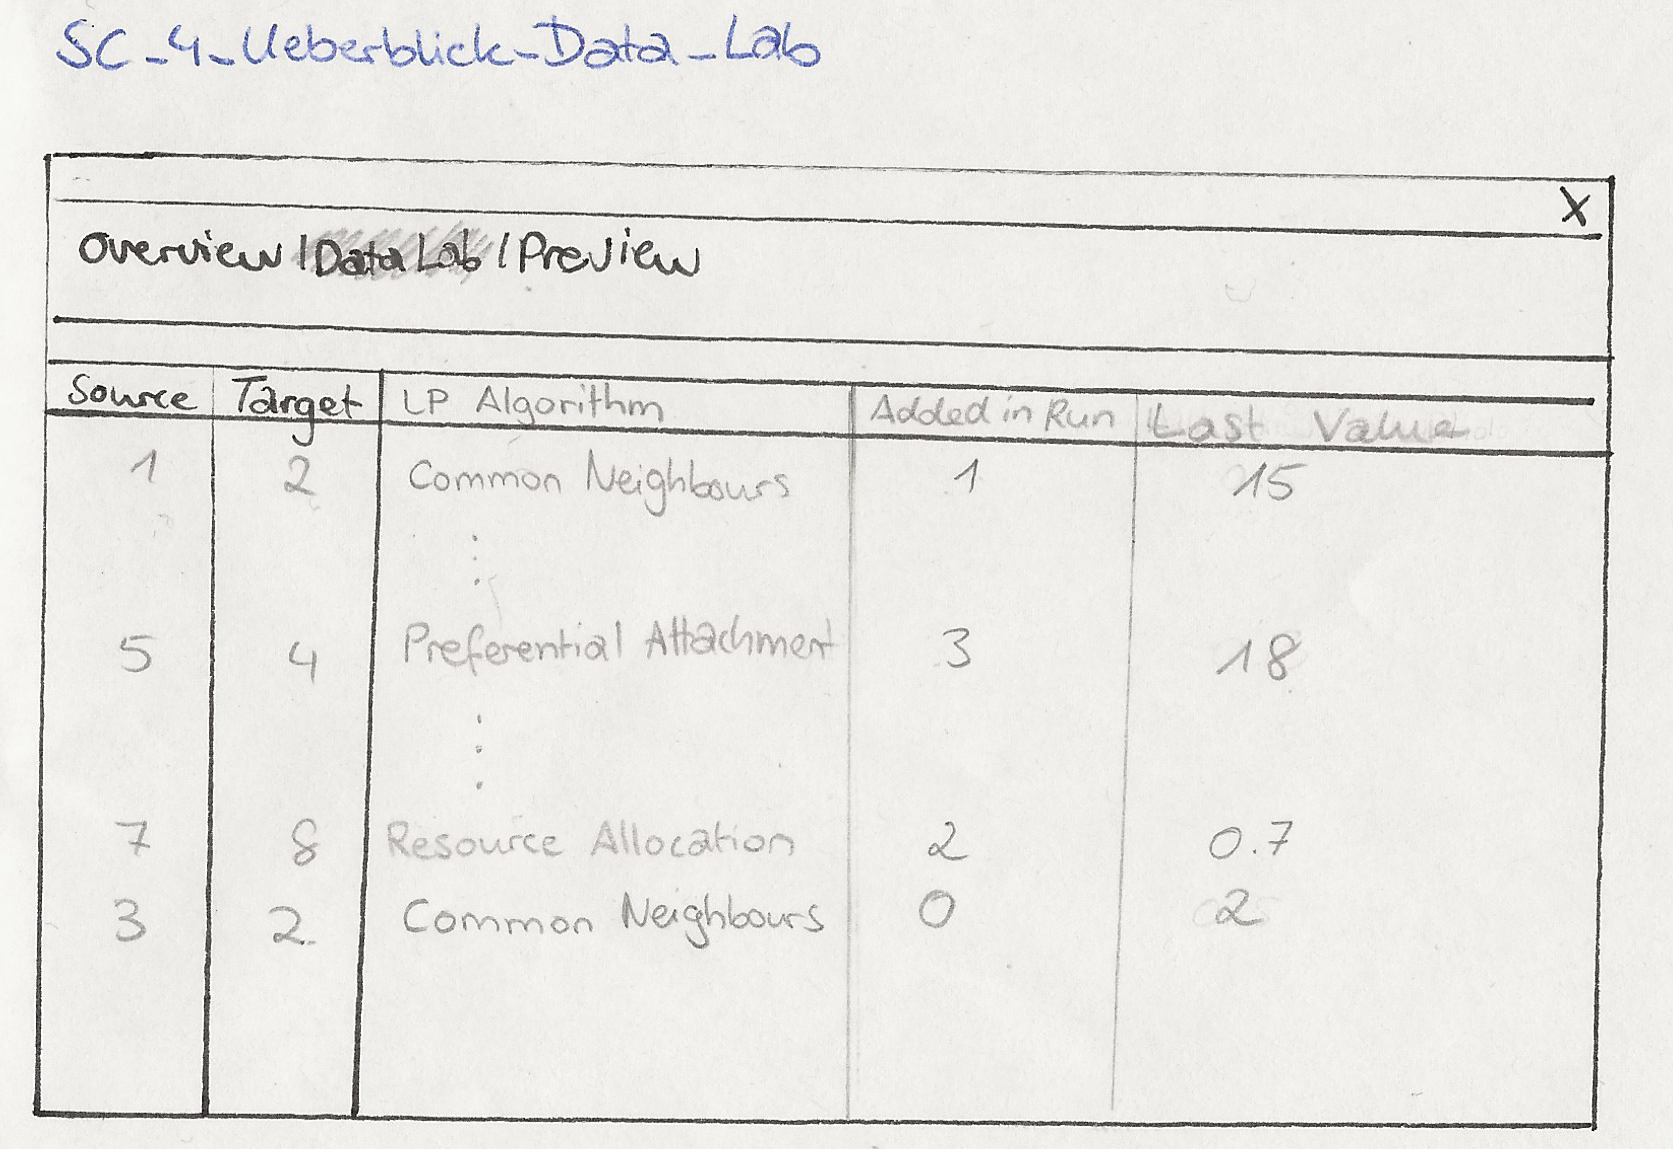
\includegraphics[width=\linewidth]{resources/SC-4.png}
    \caption{Data Laboratory mit neuen Edges.}
    \label{fig:screen4}
\end{figure}

Abbildung \ref{fig:screen4} zeigt die neuen Kanten im \ovalbox{Data Laboratory}.
Wie bereits erwähnt, wurden den Kanten neue Attribute hinzugefügt.
% TODO: Heisst in impl neu anders?
Neu gibt es ein Attribut ``Link Prediction Algorithm'', in welchem ersichtlich ist, mit welchem Algorithmus die Kante hinzugefügt wurde.
Falls das Attribut keinen Wert enthält, war die Spalte bereits im initialen Graphen vorhanden.

Eine weiteres Attribut ist ``Added in Run''. Gibt der User bei der Berechnung den Wert $3$ mit, so werden hier 3 Kanten pro
ausgewähltem Algorithmus nacheinander hinzugefügt. Damit nachträglich erstlichich ist, in welchem Durchlauf eine
Kante hinzugefügt wurde, wird der Iterationsdurchgang in diesem Attribut persisiert.
Ein Wert von $1$ bedeuted demnach, dass die Kante in der ersten Iteration hinzugefügt wurde, währen ein Wert von $3$ bedeutet, dass die Kante im dritten Durchlauf zum Graphen hinzugefügt wurde.
Kanten, die bereits im initialen Graphen vorhanden waren, enthalten keinen Wert in dieser Spalte.

Bei der dritten zusätzlichen Spalte "Last Value" wird der letzte berechnete Wert einer neu hinzugefügten Spalte eingetragen.
Damit kann nachträglich einfach nachvollzogen werden, aufgrund welcher Wahrscheinlichkeit eine Kante zum Graphen hinzugefügt wurde.
Bei Kanten, die im initialen Graphen bereits vorhanden waren, ist dieses Attribut wiederum leer.

\subsection{Filtern vorhergesagter Kanten}

Die neu hinzugefügten Kanten sollen gefiltert werden können.
Der folgende Abschnitt veranschaulicht, wie die Funktionlität im Gephi Plugin visualisiert wird.

\begin{figure}
    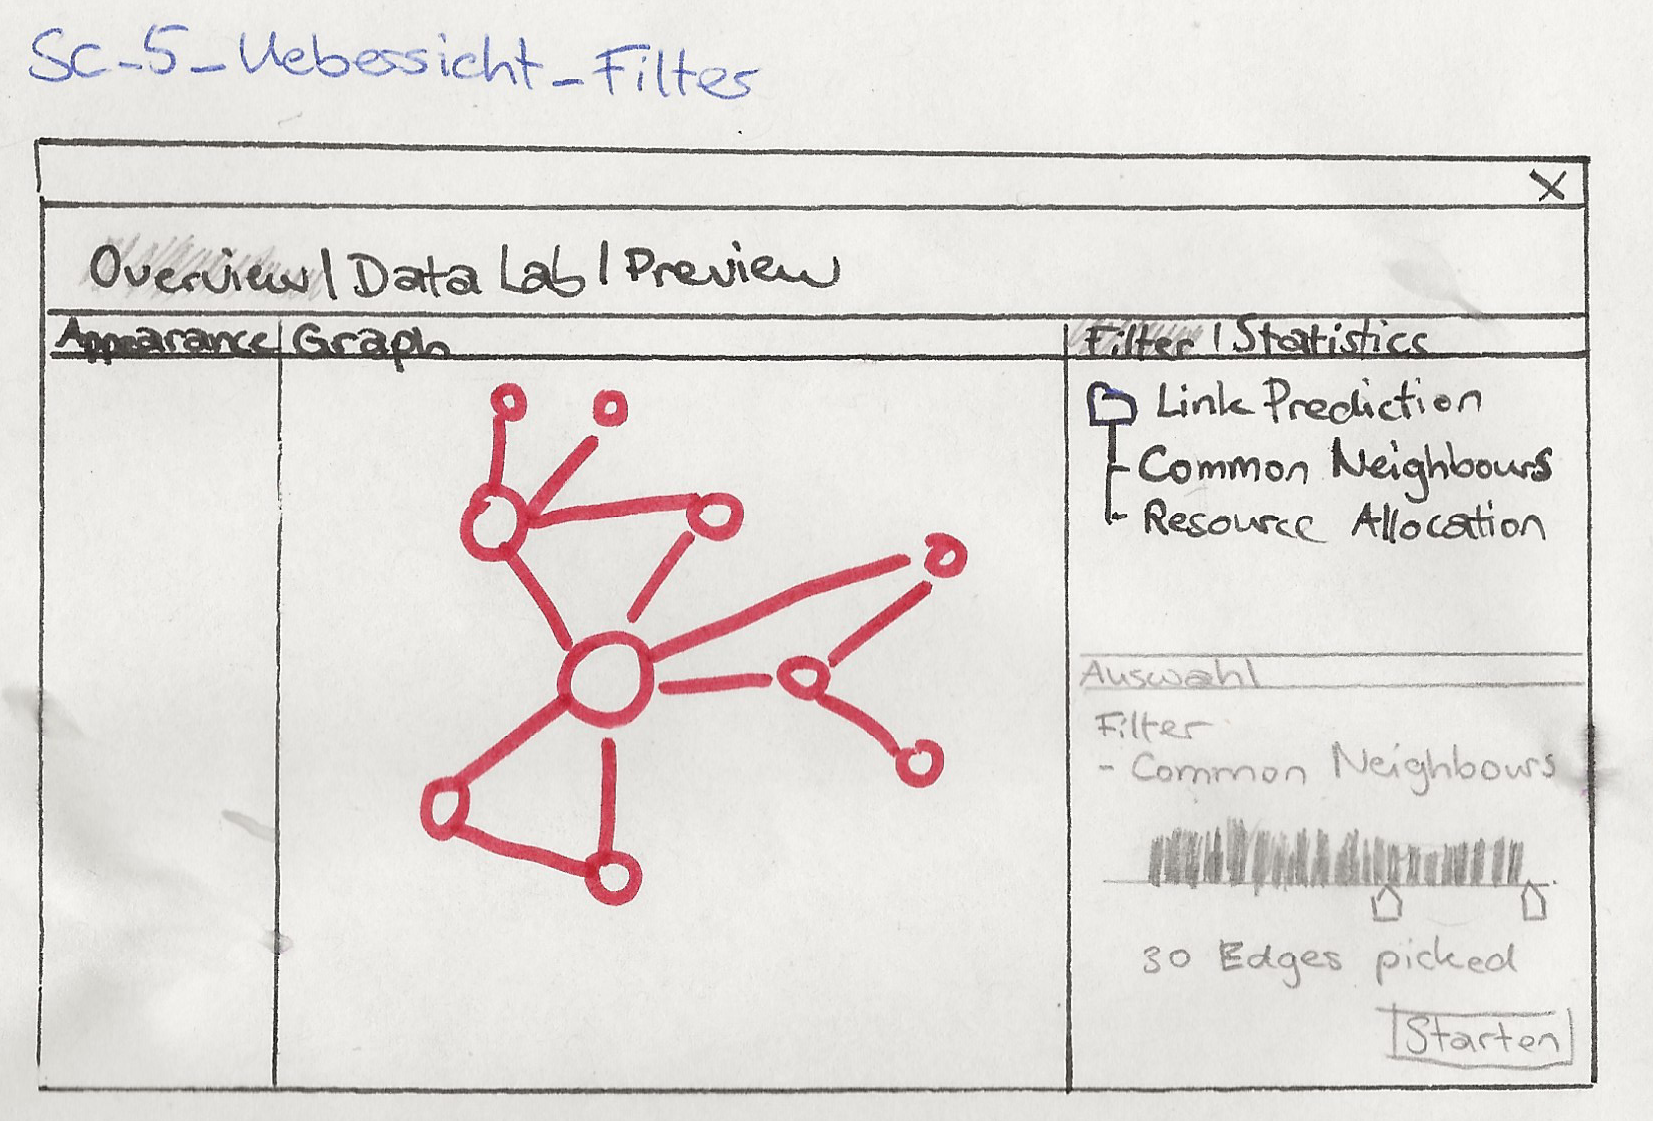
\includegraphics[width=\linewidth]{resources/SC-5.png}
    \caption{Überblick der Ansicht Filter.}
    \label{fig:screen5}
\end{figure}

In Abbilung \ref{fig:screen5} istzu sehen, wie der Link Prediction Filter in die bestehende Übersicht eingebunden wird.
Unter der Schaltfläche \ovalbox{Filter} gibt es eine neue Kategorie ``Link Predictions''.
Darin werden die Filter für die verschiedenen Algorithmen aufgeführt.
Mithilfe eines grafischen Elements kann konfiguriert werden, welche Kanten des jeweiligen Algorithmus angezeigt werden sollen.
Durch Positionieren des Sliders können alle Kanten ausgewählt werden, welche in einem gewünschten Iterationrange zum Graphen hinzugefügt wurden.
Der Filter wird durch Anwählen der Schaltfläche \ovalbox{Start} angewendet.

Falls für den spezifischen Algorithmus noch keine Kanten zum Graphen hinzugefügt wurden, erscheint ein Pop-up Fenster mit entsprechendem Hinweis.
Abbildung \ref{fig:screen6} zeigt das Pop-up Fenster.

\begin{figure}
    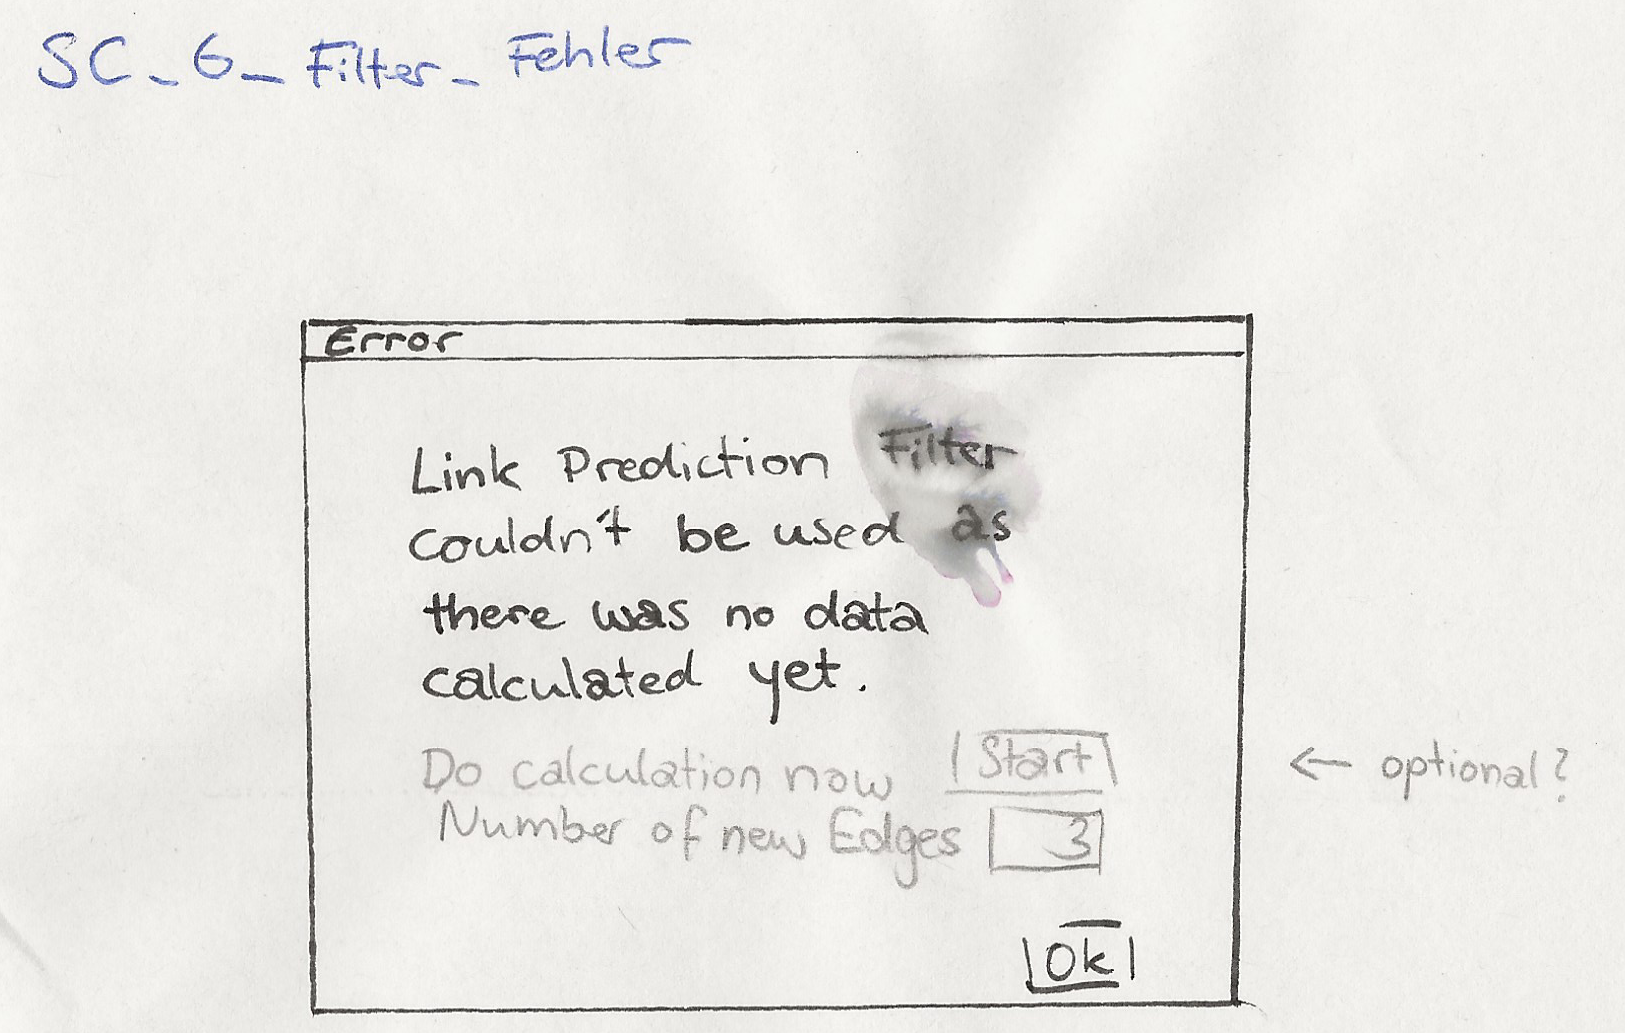
\includegraphics[width=\linewidth]{resources/SC-6.png}
    \caption{Fehlermeldung, wenn die Berechnung der Link Prediction noch nicht durchgeführt wurde.}
    \label{fig:screen6}
\end{figure}

Der Platzhalter ``Link Prediction Filter'' wird durch den gewählten Algorithmus, z.B. ``Common Neighbour Filter'' ersetzt.
Ursprünglich war angedacht, dass im Fehlerfall die Berechnung direkt aus dem Pop-up Fenster angestossen werden soll.
Um die Trennung zwischen den beiden Konzepten \textit{Filter} und \textit{Statistik} klar zu halten, wurde darauf verzichtet.
Die notwendige Berechnung kann weiterhin über \ovalbox{Statistics} vorgenommen werden (vgl. voriger Abschnitt).

Abbildung \ref{fig:screen7} zeigt den gefilterten Graph. Er enthält alle Kanten, welche mit dem gewählten Algorithmus hinzugefügt wurden und
innerhalb der konfigurierten Iterationswerte liegen.
% TODO: Initiale Kanten?

\begin{figure}
    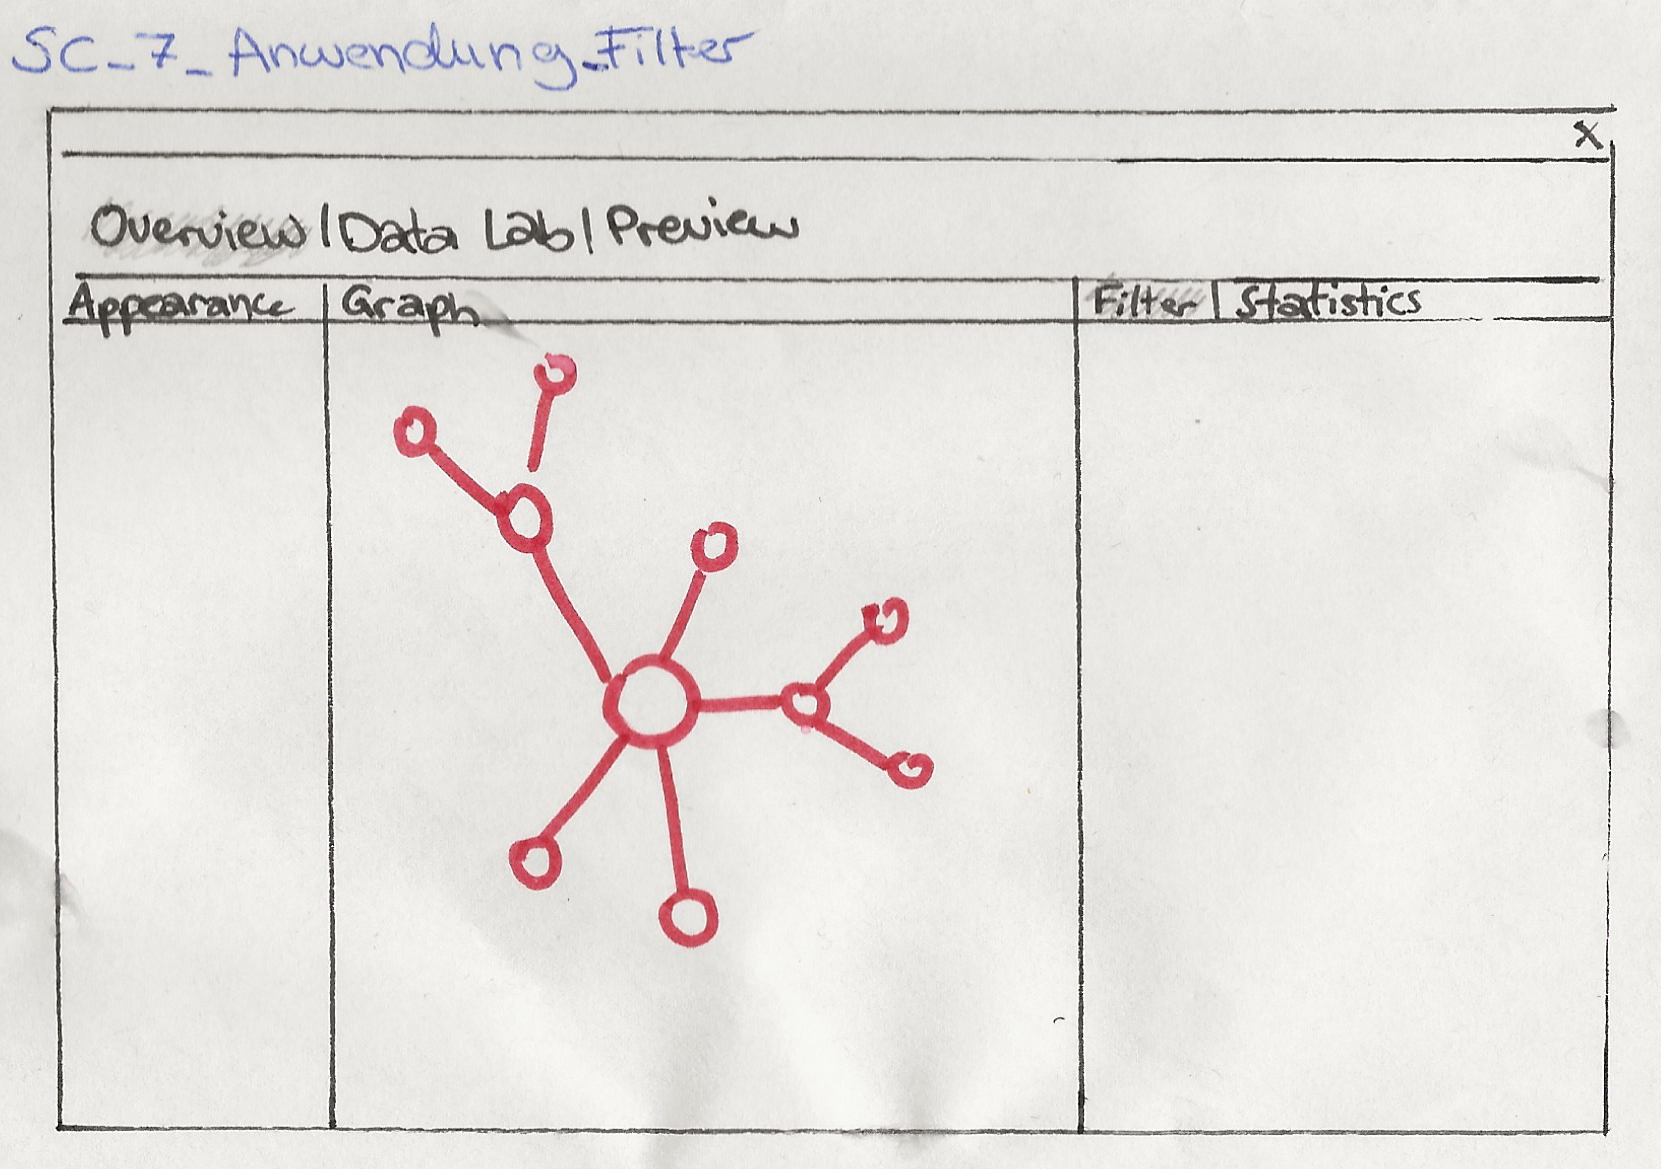
\includegraphics[width=\linewidth]{resources/SC-7.png}
    \caption{Gefilterter Graph.}
    \label{fig:screen7}
\end{figure}

\subsection{Beurteilung der Qualität verschiedener Algorithmen}

Dummy text.


\section{Anleitung Software}

Eine Anleitung der Software befindet sich im Anhang \ref{readme} in Form des README.md.

%
%
%Nach Recherche über die verschiedenen Algorithmen wurde entschieden, die Algorithmen "Common Neighbours" und
%"Preferential Attachment" zu implementieren. Diese Entscheidung beruhte darauf, dass sich die beiden Algorithmen
%insofern unterscheiden, dass beim Common-Neighbours-Algorithmus nur Knoten eine Rolle spielen, welche gemeinsame
%Nachbarn aufweisen. Beim zweiten Algorithmus ist dies anders: Dort werden alle Knoten im Bezug aufeinander
%berücksichtigt - hier ist also die Popularität eines einzelnen entscheidend, während beim ersteren Gemeinsamkeiten im
%Vordergrund stehen.
%
%In der Literatur werden hauptsächlich Algorithmen beschrieben, welche auf ungerichtete Graphen anwendbar sind. Algorithmen für gerichtete Graphen weisen eine wesentlich höhere Komplexität auf. Die Arbeit beschränkt sich deshalb auf Link Predictions auf ungerichtete Graphen -
%ein entsprechender Hinweis wurde im Gephi Plugin implementiert.
%
%\subsection{Common Neighbours}
%In Gephi ist die Berechnung dieses Werts bei den Statistiken unter Link Prediction zu finden. Die berechneten Werte
%werden anschliessend im Data Laboratory gespeichert und können mit Hilfe von Filtern eingeschränkt werden.
%
%\begin{figure}[htbp]
%    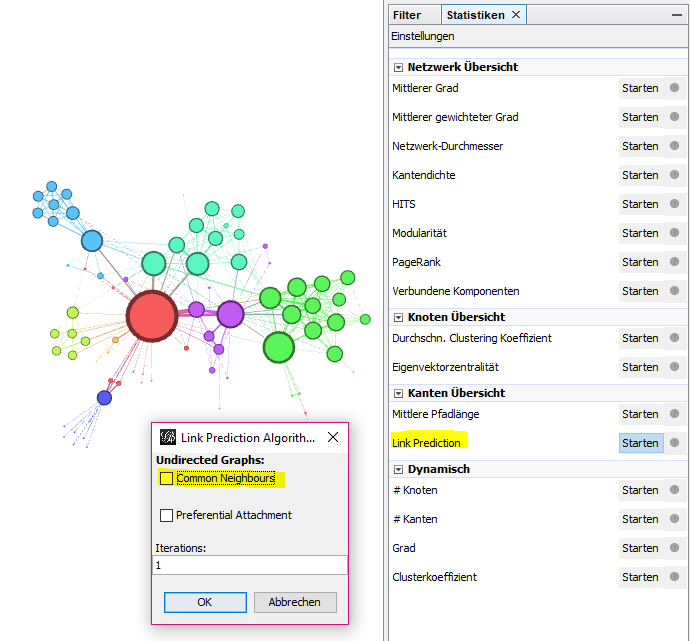
\includegraphics[width=\linewidth]{resources/gephi-CN.png}
%    \caption{Gephi Common Neighbours Funktion.}
%    \label{fig:screen8}
%\end{figure}
%
%\subsection{Preferential Attachment}
%In Gephi ist die Berechnung dieses Werts bei den Statistiken unter Link Prediction zu finden. Die berechneten Werte
%werden anschliessend im Data Laboratory gespeichert und können mit Hilfe von Filtern eingeschränkt werden.
%
%\begin{figure}[htbp]
%    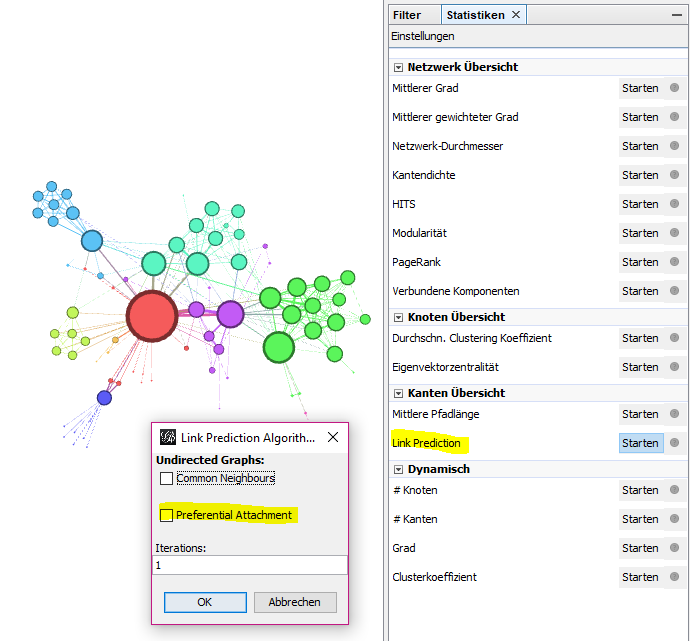
\includegraphics[width=\linewidth]{resources/gephi-PA.png}
%    \caption{Gephi Preferential Attachment Funktion.}
%    \label{fig:screen9}
%\end{figure}
%
%\section{Evaluationskomponente}
%
%Dummy text.
%
